\begin{figure}
\centering
\begin{tikzpicture}[
    node distance=2cm,
    every node/.style={font=\normalsize},
    mycircle/.style={circle, draw=black, thick, minimum size=1cm, inner sep=1pt},
    myarrow/.style={-{Stealth[length=3mm, width=2mm]}, thick}
]
% Left node
\node[mycircle] (start) at (0.025\textwidth + 0.45cm,0) {$x_0$};
% Right node — placed at the right edge of the text width
\node[mycircle] (end) at (0.975\textwidth-1.45cm, 0) {$x_{t_L}$};
% Arrow connecting them
\draw[myarrow] (start) -- (end);
% Equation overlaying the line with rounded rectangle background
\node[fill=gray!10, draw=black, thick, rounded corners=3pt, inner sep=4pt, align=center] at ($(start)!0.5!(end)$) {
$dx_t = \left[-a(t)x_t + \sigma(t)^2 \ \smash{
    \overbrace{\mathbf{f}_\theta\!\left(t,x_t,t_{i^*+1}, \mathbf{x}_{0:i^*}\right)}^{\mathclap{\substack{
        \text{path-dependent score, minimizer of \eqref{eqn:simplified_dsm_main}}
        }}
    }
} \ \right]dt + \sigma(t)dB_t$
};
\end{tikzpicture}
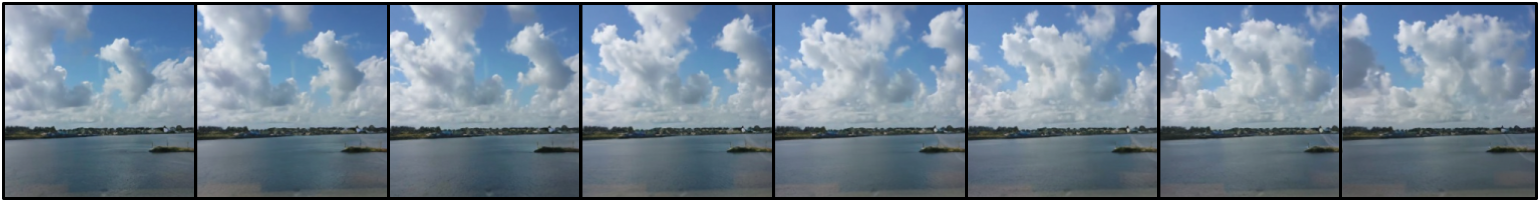
\includegraphics[width=0.95\linewidth]{diagrams/sky_frames.png}
\caption{\textbf{ABC Schematic:} The time series generation SDE from Thm. \ref{thm:new_sde} is learned via Thm. \ref{thm:path_dependent_score}. $\mathbf{f}_\theta\!\left(t,x_t,t_{i^*+1}, \mathbf{x}_{0:i^*}\right)$ is the path-dependent score (parameterized by neural net), $\mathbf{x}_{0:i^*}$ is the conditioning frame history, $t$ is the current \textit{physical} time, $t_{i^*+1}$ is the next frame's physical time.}
\end{figure}
